\documentclass[12pt]{article}

\usepackage{cite}
\usepackage{amsmath,amssymb,amsfonts}
\usepackage{algorithmic}
\usepackage{graphicx}
\usepackage{textcomp}
\usepackage{xcolor}
\usepackage{float}
\usepackage{subfigure}
\usepackage{listings}
\usepackage{color}
\usepackage{geometry}
\geometry{a4paper,left=3.5cm,right=3.5cm,top=2.5cm,bottom=2.5cm}

\definecolor{dkgreen}{rgb}{0,0.6,0}
\definecolor{gray}{rgb}{0.5,0.5,0.5}
\definecolor{mauve}{rgb}{0.58,0,0.82}

\lstset{frame=tb,
  language=Python,
  aboveskip=3mm,
  belowskip=3mm,
  showstringspaces=false,
  columns=flexible,
  basicstyle={\small\ttfamily},
  numbers=none,
  numberstyle=\tiny\color{gray},
  keywordstyle=\color{blue},
  commentstyle=\color{dkgreen},
  stringstyle=\color{mauve},
  breaklines=true,
  breakatwhitespace=true,
  tabsize=3
}

\begin{document}

\title{\textbf{Gesture Recognition Based On Deep Learning}}
\author{Runlin Hou \and Sifan Yuan \and Yuxiang Song \and Haocong Wang}
\maketitle

\begin{abstract}
Gesture recognition is a topic in computer science, mainly talking about making computers recognize human body movements. It can be captured from all parts of human body, but it mainly comes from faces and hands. In our project, we focus on hand movements. In order to present a better result, we choose gestures of numbers as our training and testing object. Our project is based on PyTorch, an open source machine learning library. We choose LeNet and ResNet as the network of the model and compare the performance between the two networks. Finally, we implement a product using our trained model to evaluate its feasibility.
\end{abstract}

\section{Introduction}
Gesture recognition is a vital approach to make the direct communication between human and computers achievable without extra mechanical devices compared to primitive text user interfaces and traditional GUI. It can be widely utilized in applications, such as virtual reality and sign language. In our daily lives, we already contact with gesture recognition in a high frequency. For example, one of the commonly used electronic devices, iPad, supports gesture operation, which requires the ability of gesture recognition. Gesture recognition has a broad range of applications in human-computer interaction. For example, in virtual reality and augmented reality, gesture recognition can be applied widely. Also, in the smart home domain, gesture recognition can be utilized to remotely control smart appliances and home robots. It can be conducted with techniques from computer vision and image processing.

LeNet, one of the oldest CNNs, was created in 1994. By convolution, sharing parameters and pooling, LeNet is able to categorize and recognize patterns using fully connected neural networks without high costs. It has been the start point of various networks developed later. The Residual Neural Network (ResNet) was proposed by Kaiming He, which solved the degradation problem of deep neural networks using residual learning. ResNet adds skip connection in the networks between layers, which makes the network only need to learn the different part between the input and output, simplifying the learning process. The detailed description of our proposed LeNet and ResNet will be given in the model section.


\section{Dataset}

We load two datasets in our system  which are Sign Language MNIST and Kinect Leap Dataset. The original MNIST image dataset of handwritten digits is a popular benchmark for image-based machine learning methods, the dataset format is patterned to match closely with the classic MNIST. Each training and test case represents a label (0-25) as a one-to-one map for each alphabetic letter A-Z (and no cases for 9=J or 25=Z because of gesture motions). The training data (27,455 cases) and test data (7172 cases) are approximately half the size of the standard MNIST but otherwise similar with a header row of label, pixel1, pixel2 …. pixel784 which represent a single 28x28 pixel image with grayscale values between 0-255. The second one is Microsoft Kinect and leap motion. The database contains 10 different gestures performed by 14 different people. Each gesture is repeated 10 times for a total of 1400 different data samples. For each sample, Leap Motion data have been acquired together with the depth maps and color images provided by the Kinect. This dataset includes 10 gestures which represent the number 1-10.
\section{Model}
In this section, we will have a brief introduction of the two networks we use in the project.

\subsection{LeNet5}
Structure of LeNet5 is: input layer$\rightarrow$ convulational layer$\rightarrow$pooling layer$\rightarrow$ activation function$\rightarrow$ convulational layer$\rightarrow$ pooling layer$\rightarrow$ activation function$\rightarrow$ convulational layer$\rightarrow$ fully connect layer$\rightarrow$ fully connect layer$\rightarrow$ output layer.

\begin{figure}[H]
    \centering
    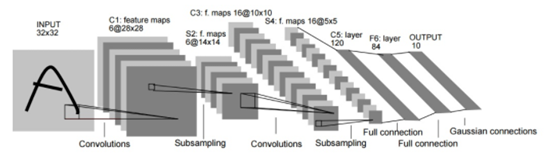
\includegraphics[scale=0.9]{modelpic/LeNet.png}
    \caption{LeNet5}
\end{figure}

\begin{itemize}
    \item Input layer, The input is pixel picture whose size been $28\times 28$
    \item C1 layer, convolutional layer with kernel size been $5\times 5$
    \item S2 layer, downsampling layer to extract the image attributes
    \item C3 layer, convolutional layer with kernel size also been $5\times 5$
    \item S4 layer, another downsampling layer 
    \item C5 layer, convolutional layer with kernel size been $5\times 5$
    \item F6 layer, fully connected layer with output usually been 10, to make the final prediction
    \item Output layer, pick up ouput with highest probability
\end{itemize}

\subsection{ResNet34}
The second network we use is ResNet. According to the universal approximation theorem, given enough capacity, we know that a feedforward network with a single layer is sufficient to represent any function. However, the layer might be massive and the network is prone to overfitting the data. Therefore, there is a common trend in the research community that our network architecture needs to go deeper. But when the network goes deeper, the result and may not be so well because a lot of problem raising by the depth of the network. Two kinds of problem, the gradient exploding and vanishing, has been successfully addressed. The ResNet here is to solve the information loss during the process when networks become deeper and deeper. The main idea is to make identity mapping possible. Instead of finding the output, the ResNet focus on the residual part. It uses a shortcut to connect the layers, to feed the original input to the residual output to get the final output answer. Using this method can reduce the information loss during the mapping, because we can get the original input as the output even if the network didn’t work well.

\begin{figure}[H]
    \centering
    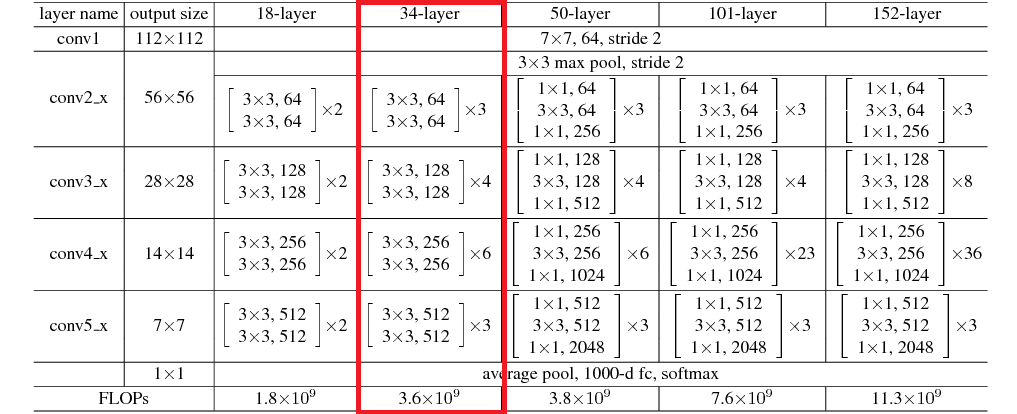
\includegraphics[scale = 0.9]{modelpic/resnet.png}
    \caption{ResNet34}
    \label{}
\end{figure}



\section{Implementaion}
In this section, we are going to talk about how we implement the network and training process. We seperatet this section into three parts according to the code, which corresponding to implement the models, resizing of the dataset, and the whole training process.
\subsection{Model Implementation}
For our project, we implement two classic CNN models, which are LeNet5 and ResNet34. As we mentioned above, LeNet5 is a simple CNN model with 7 layers, which is relatively small compared to ResNet34. And of course, a smaller size of the model always corresponding to a relatively poorer performance. With a larger scale, ResNet34 can deal with more parameters and consequently results in a better capability to a larger scale image. And we will show a more detailed test result in the next section.
\subsubsection*{LeNet5}
There is only 7 layers (exclusion of the input layer) in the LeNet5, so we can easily implement layer by layer with Pytorch. In section 3 we mentioned that LeNet5 is consist of convolutional layers and fully connected layers, which all have their packged function in Pytorch. 

But for our project something we need to pay attention to is that the input channel of the first convolutional layer. Since we have two dataset to train on and one of them is an RGB dataset, but the original LeNet5 is designed for gray scale image, we need to make the LeNet5 enable to deal with the 3-channel RGB images. Therefore, we adjust the input channel according to the input dataset. Also, the dataset does not share same amount of classes included, which means the final output also needed to be matched with dataset.

\begin{lstlisting}
  class LeNet5(nn.Module):
    def __init__(self, class_num, is_gray_scale):
        super(LeNet5, self).__init__()

        if is_gray_scale:
            input_channel = 1
        else:
            input_channel = 3

    ......

    def num_flat_features(self, x):
        size = x.size()[1:]
        num_features = 1
        for s in size:
            num_features *= s
        return num_features
\end{lstlisting}

\subsubsection*{ResNet34}
Since ResNet34 got a much more complex structure compared to LeNet5 and includes a repetive structure called residual block, we will implement the residual block first to simplify the code. As we mentioned in section 3, a classic residual block always consist of two convolutional layers with batchnorm process between. Also, in the forward computing process, the key of residual network is to add $x$ to the layer output $H(x)$ to get $H(x)+x$ to compute the residual. Following the typically methods, we implement this residual block.
\begin{lstlisting}
  class ResBlock(nn.Module):
    def __init__(self, inchannel, outchannel, stride=1, shortcut=None):
        super(ResBlock, self).__init__()
        self.basic = nn.Sequential(
            nn.Conv2d(inchannel, outchannel, 3, stride, 1, bias=False),
            nn.BatchNorm2d(outchannel),
            nn.ReLU(inplace=True),
            nn.Conv2d(outchannel, outchannel, 3, 1, 1, bias=False),
            nn.BatchNorm2d(outchannel),
        )
        self.shortcut = shortcut

    def forward(self, x):
        out = self.basic(x)
        residual = x if self.shortcut is None else self.shortcut(x)
        out += residual
        return nn.ReLU(inplace=True)(out)
\end{lstlisting}

\begin{figure}[H]
    \centering
    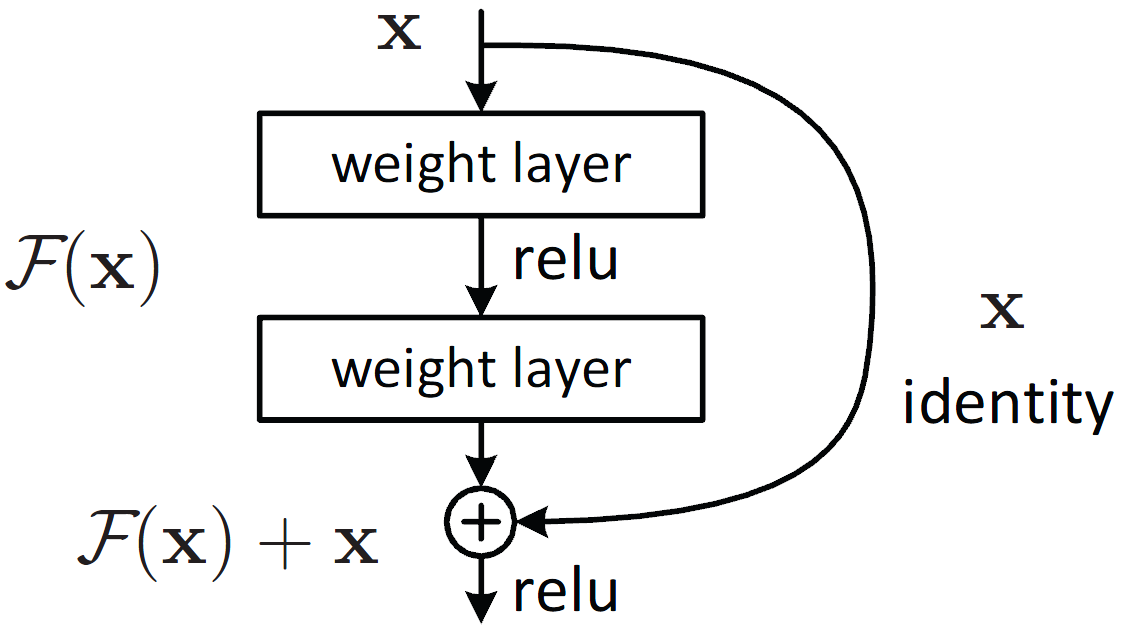
\includegraphics[scale=0.3]{modelpic/ResBlock.png}
    \caption{Residual Block}
    \label{}
\end{figure}

After we got the residual block class, we can construct the whole network by the superposition of multiple residual blocks. In our project we choose to implement a 34-layer residual network. Before the residual learning process, we first have a convolutional layer for the normalize of the input images to make them fit the subsequent residual block layers. Then we have 4 groups of residual block layers. The first layer have 3 residual blocks with 64 input channels and 128 output channels. The second layer has 4 residual blocks with 128 input channels and 256 output channels. The third layer has 6 residual block with 256 input channels and 512 output channels. The fourth layer has 3 residual blcok with 512 input channels and 512 output channels. Then the network end up with a fully connected layer for the prediction result. So the network has 1 initial convolutional layer and 32 convolutional layers in residual block and one last fully connected layer for output prediction, which are 34 layers in total.

Similarly with LeNet5, our project requires the network to fit the two datasets we have. Also, we want to test how the model work on the gray scale images compared to RGB images. To achieve this requirement, we have the input channel of the first convolutional layer and the output of the last fully connected layer to be adjustable. 

\begin{lstlisting}
  class ResNet34(nn.Module):
    def __init__(self, class_num, is_gray_scale):
        super(ResNet34, self).__init__()
        if is_gray_scale:
            input_channel = 1
        else:
            input_channel = 3

        self.pre = nn.Sequential(
            nn.Conv2d(input_channel, 64, 7, 2, 3, bias=False),
            nn.BatchNorm2d(64),
            nn.ReLU(inplace=True),
            nn.MaxPool2d(3, 2, 1),)
        self.layer1 = self.__make_layer__(64, 128, 3)
        self.layer2 = self.__make_layer__(128, 256, 4, stride=2)
        self.layer3 = self.__make_layer__(256, 512, 6, stride=2)
        self.layer4 = self.__make_layer__(512, 512, 3, stride=2)
        self.fc = nn.Linear(512, class_num)
        ......

    def forward(self, x):
        ......

        return self.fc(x)
\end{lstlisting}

\subsection{Datasets Adjustment}
In our project, we have two datasets for training as we mentioned in section 2. The first one is sign language mnist dataset, the amount of this dataset are huge compared to the kinect leap dataset. Since this dataset is actually designed for the LeNet, the size of images inside the dataset is $28\times 28$, which is relatively small compared to the other one. This make us a problem that the images are too small for the ResNet34, the images are unacceptable for ResNet34 since the images are smaller than a convolutional core of the first convolutional layre. Meanwhile, LeNet5 can neither learning an image with too large scale. So the main purpose of this part is to deal with the size of the input images. Considering all the requirements mentioned above, we choose to resize the image to $224 \times 224$ for ResNet34 and $28\times 28$ for LeNet5.

Also, another factor we want to experiment on is that he whether the gray scale of the the image influenced the training result. To fullfill this purpose we add a trigger to the dataset dealing process, which allow us to choose to output the images in 1 channel our 3 channels. 

\begin{lstlisting}
  class dataset_loader:
    ......

    def load_sign_mnist(self, img_size, isGrayScale):
        ......

    def load_kinect_leap(self, img_size, isGrayScale, train_size=1200):
        all_data = self.load_kinect_leap_dataset()
        shuffle(all_data)

        # set train and test set
        train_data = all_data[0:train_size - 1]
        train_set = KinectLeapDataset(train_data, img_size=img_size, is_gray_scale=isGrayScale)
        train_loader = DataLoader(dataset=train_set, batch_size=8, shuffle=False)

        test_data = all_data[train_size:len(all_data) - 1]
        test_set = KinectLeapDataset(test_data, img_size=img_size, is_gray_scale=isGrayScale)
        test_loader = DataLoader(dataset=test_set, batch_size=8, shuffle=False)

        return train_loader, test_loader

    def load_kinect_leap_dataset(self):
        ......
    
  class KinectLeapDataset(Dataset):
    def __init__(self, data, img_size, is_gray_scale=False):
        print('loading kinect_leap_dataset')

        self.data = data
        self.labels = []
        self.is_gray_scale = is_gray_scale
        for label_tp in self.data:
            self.labels.append(label_tp[0])

        self.height = img_size
        self.width = img_size
        self.transform = transforms.Compose([transforms.ToTensor()])

    def __getitem__(self, index):
        single_image_label = self.labels[index]
        img_as_np = np.asarray(self.data[index][1])
        img_as_img = Image.fromarray(img_as_np)

        img_as_img = img_as_img.resize((self.height, self.width))

        if self.is_gray_scale:
            img_as_img = img_as_img.convert('L')

        if self.transform is not None:
            img_as_tensor = self.transform(img_as_img)

        return (img_as_tensor, single_image_label)

    def __len__(self):
        return len(self.data)
\end{lstlisting}

Here we take \verb|KinectLeapDataset| as an example, resizing process of the image is embeded in the \verb|.__getitem__()| function for each Pytorch \verb|dataset| class. Later by \verb|DataLoader()| class, we convert the dataset into certain size iterable batches of images in \verb|Tensor| format.

\subsection{Traing Process}
With all tools we needed, which are models and datasets. The training process are quite simple to build. For thr criterion and optimizer we choose to use \verb|CorssEntropyLoss| and \verb|SGD| optimizer. 

Also, we use a tool package \verb|tensorboardX| to monitor the training process, whose result is going to be shown in the next section.

\section{Test Result}
In this sectoin, we are going to talk about the result of the training process. We totally run six different settings to find out how the performance can be influenced by input dataset, gray scale of the images and network itself.

\begin{figure}[H]
    \centering

    \subfigure[Le-MNIST-gray]{
        \begin{minipage}[b]{0.3\textwidth}
            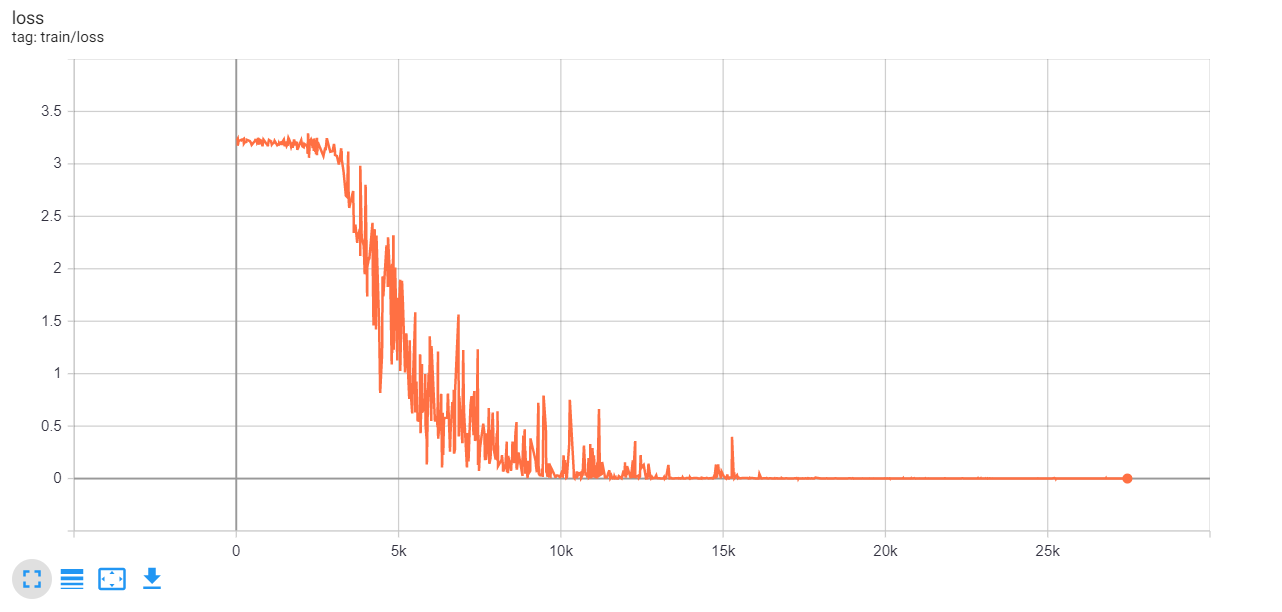
\includegraphics[width=1.1\textwidth]{pic/LeNet5GraymnistLoss.png}
        \end{minipage}
    }
    \subfigure[Le-leap-gray]{
        \begin{minipage}[b]{0.3\textwidth}
            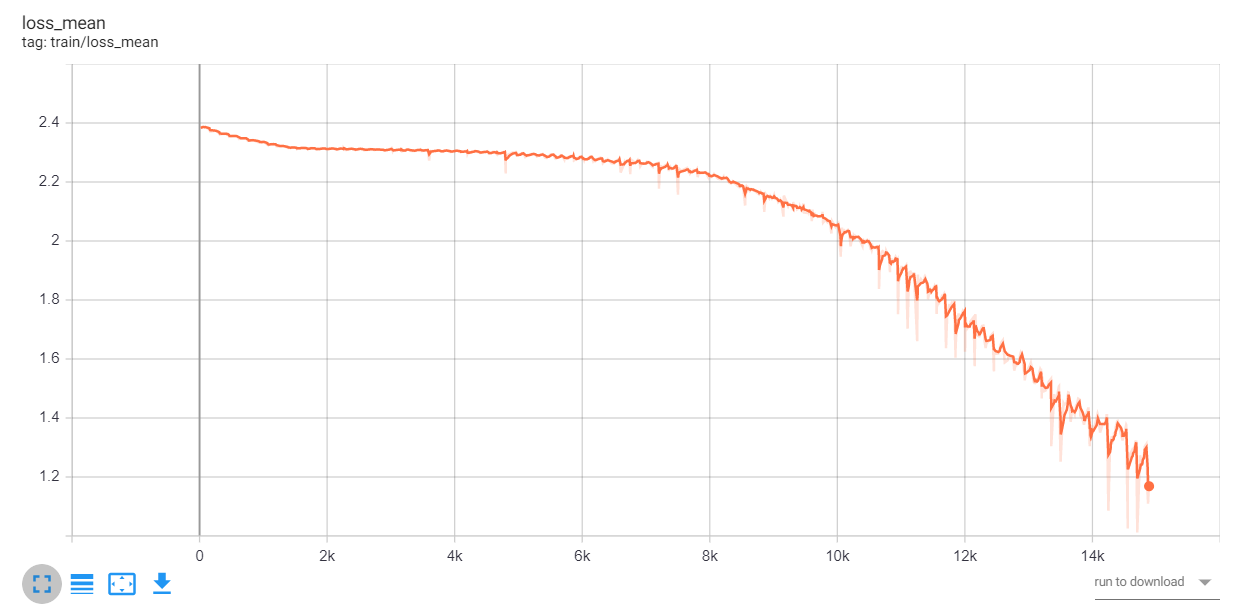
\includegraphics[width=1.1\textwidth]{pic/LeNet5grayleaploss.png}
        \end{minipage}
    }
    \subfigure[Le-leap-RGB]{
        \begin{minipage}[b]{0.3\textwidth}
            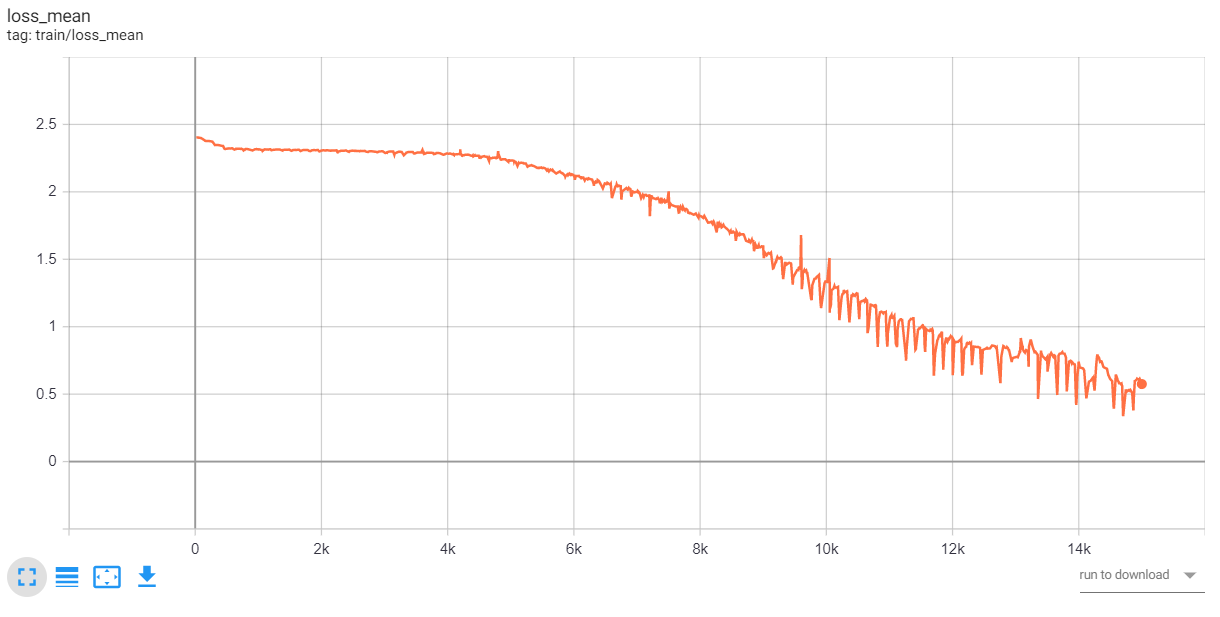
\includegraphics[width=1.\textwidth]{pic/LeNet5leaprgbloss.png}
        \end{minipage}
    }
    \\
    \subfigure[Res-MNIST-gray]{
        \begin{minipage}[b]{0.3\textwidth}
            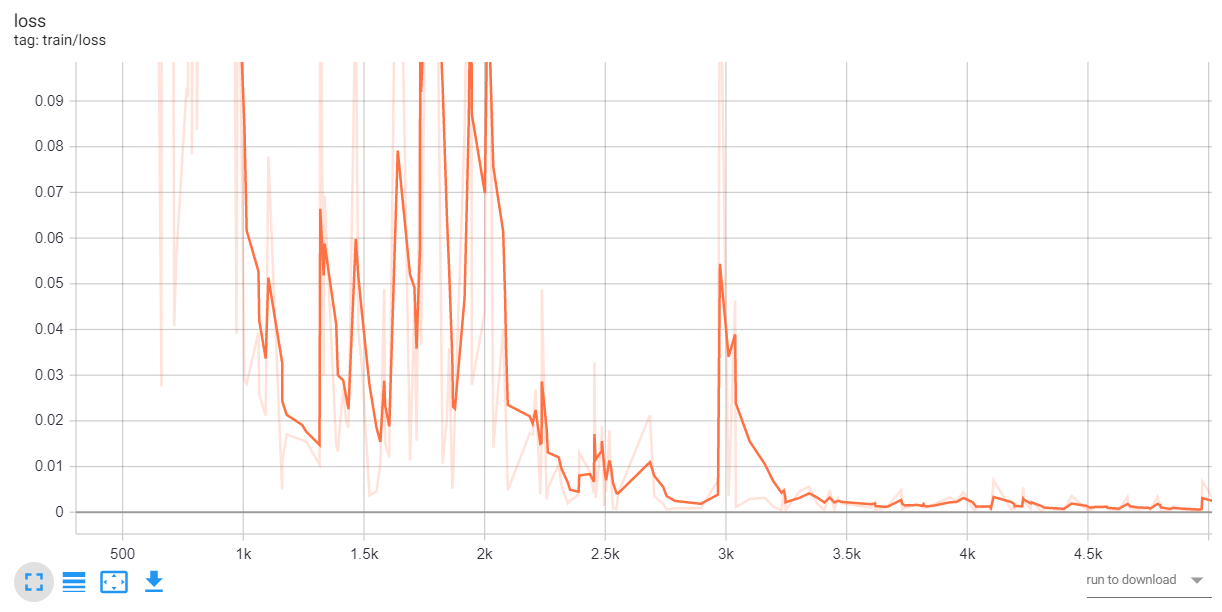
\includegraphics[width=1.1\textwidth]{pic/ResNetmnistloss.png}
        \end{minipage}
    }
    \subfigure[Res-leap-gray]{
        \begin{minipage}[b]{0.3\textwidth}
            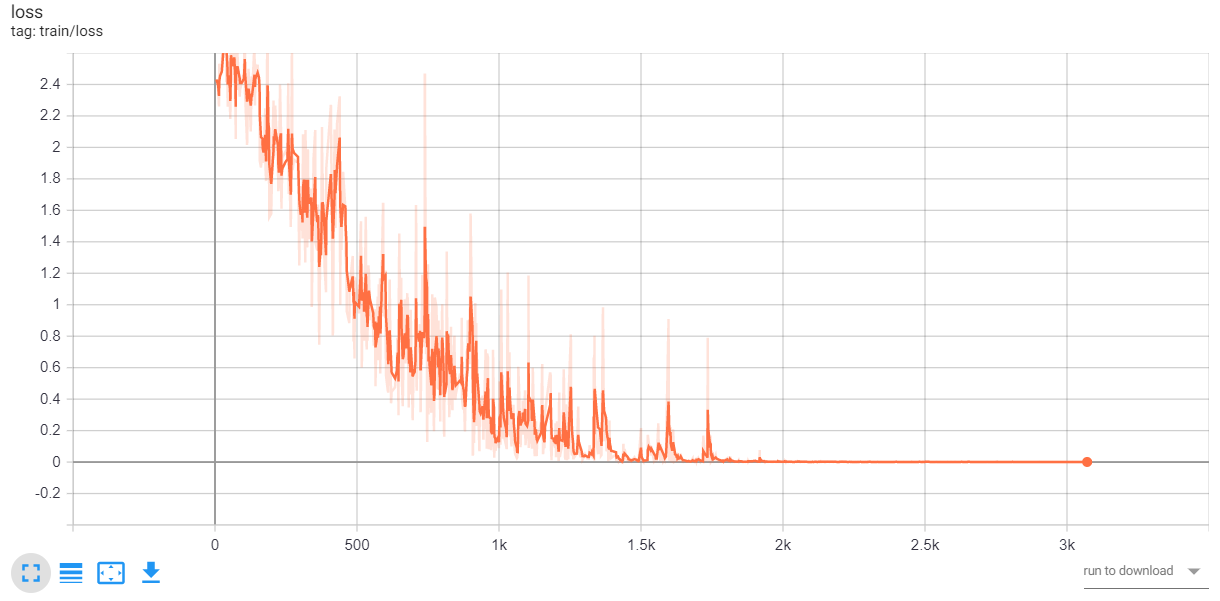
\includegraphics[width=1.1\textwidth]{pic/ResNetleaploss.png}
        \end{minipage}
    }
    \subfigure[Res-leap-RGB]{
        \begin{minipage}[b]{0.3\textwidth}
            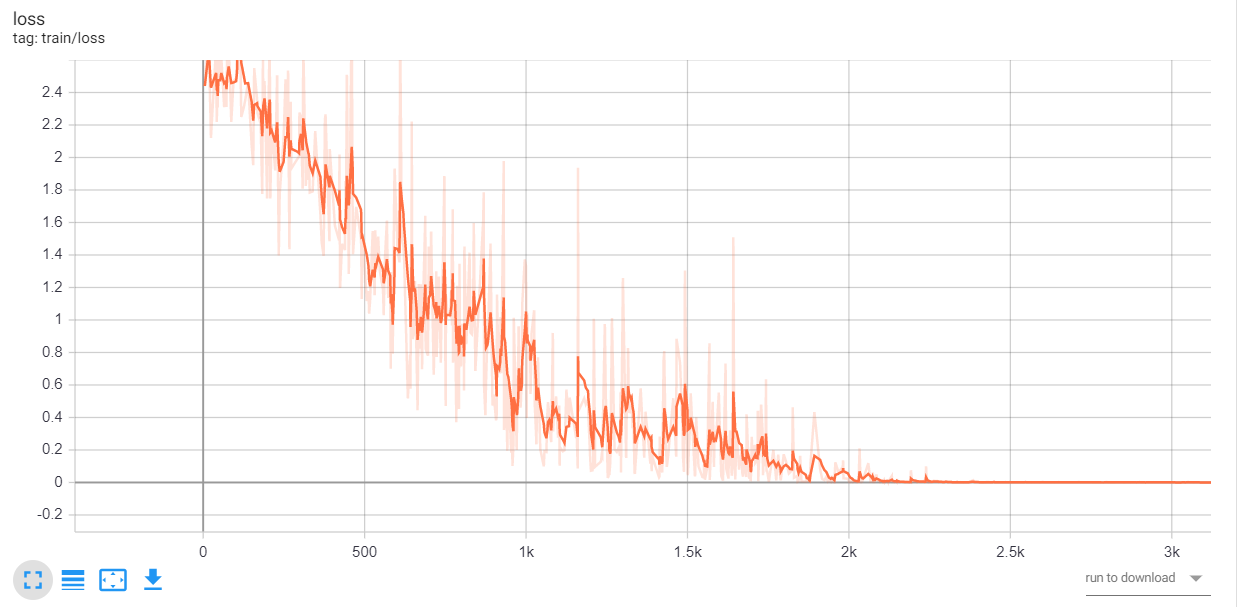
\includegraphics[width=1.1\textwidth]{pic/ResNetleaprgbloss.png}
        \end{minipage}
    }


    \caption{Variation of the loss during the training process.}
\end{figure}


\begin{figure}[H]
    \centering

    \subfigure[Le-MNIST-gray]{
        \begin{minipage}[b]{0.3\textwidth}
            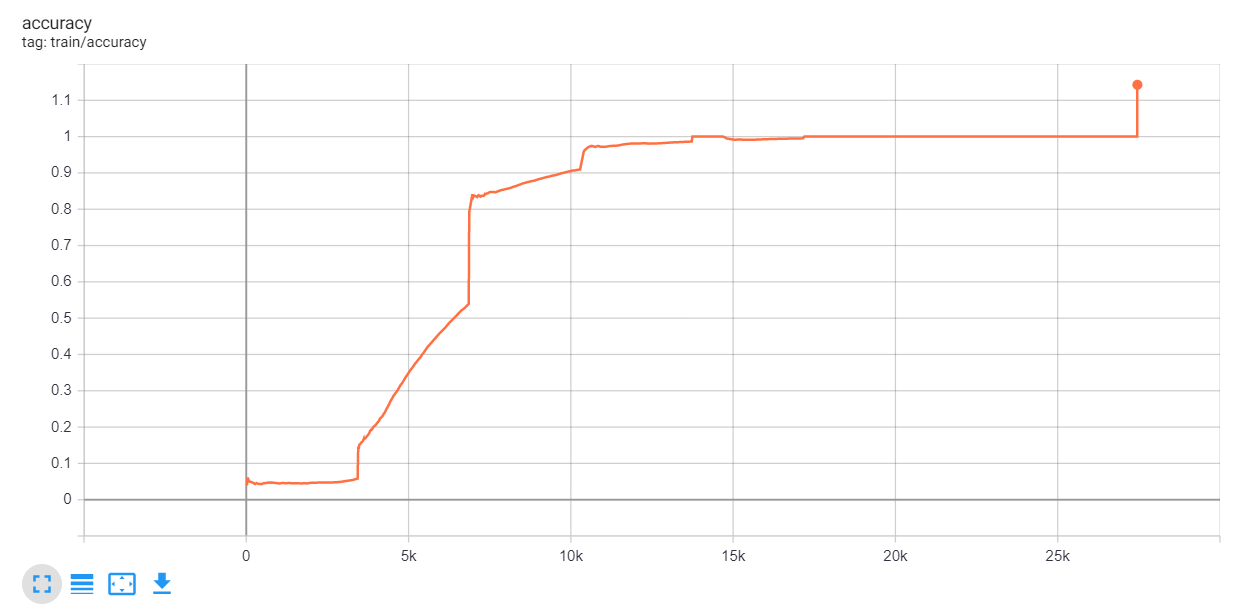
\includegraphics[width=1.1\textwidth]{pic/LeNet5Graymnist.png}
        \end{minipage}
    }
    \subfigure[Le-leap-gray]{
        \begin{minipage}[b]{0.3\textwidth}
            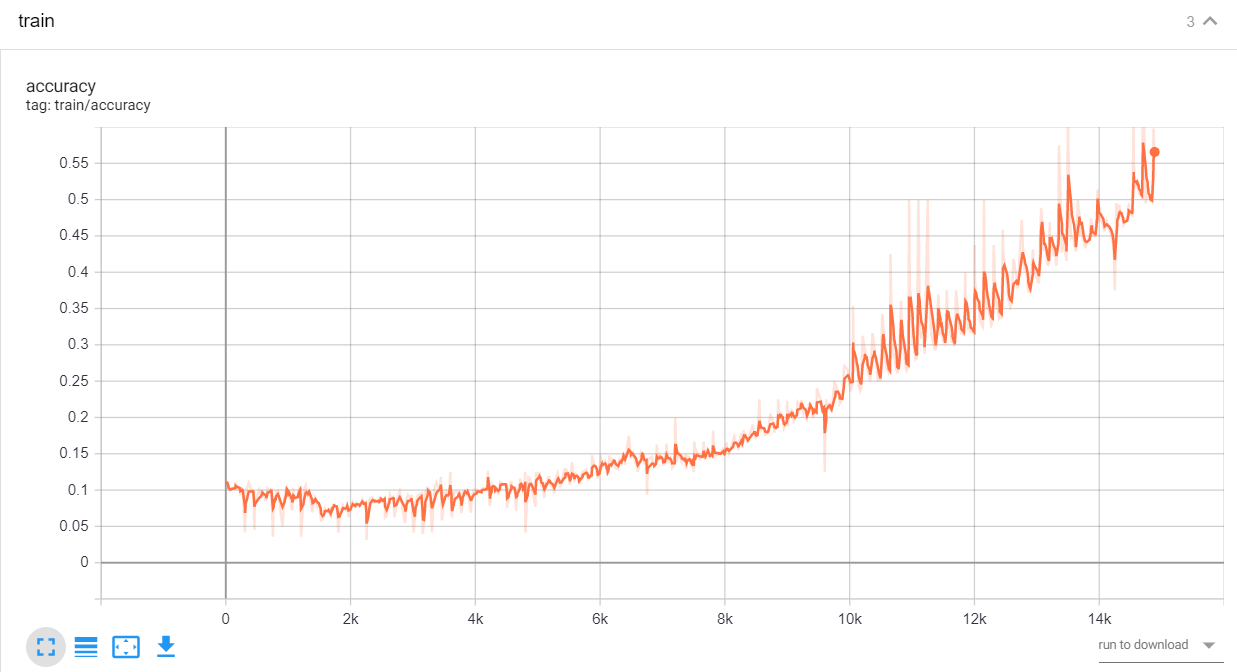
\includegraphics[width=1.1\textwidth]{pic/LeNet5grayleaptrain.png}
        \end{minipage}
    }
    \subfigure[Le-leap-RGB]{
        \begin{minipage}[b]{0.3\textwidth}
            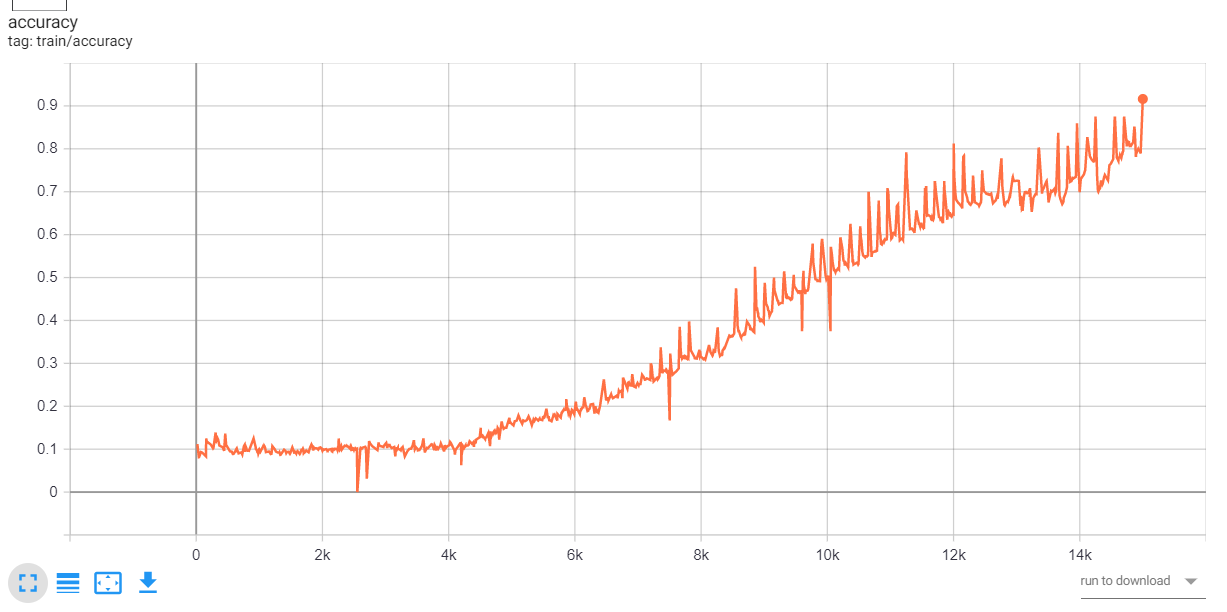
\includegraphics[width=1.\textwidth]{pic/LeNet5leaprgbtrain.png}
        \end{minipage}
    }
    \\
    \subfigure[Res-MNIST-gray]{
        \begin{minipage}[b]{0.3\textwidth}
            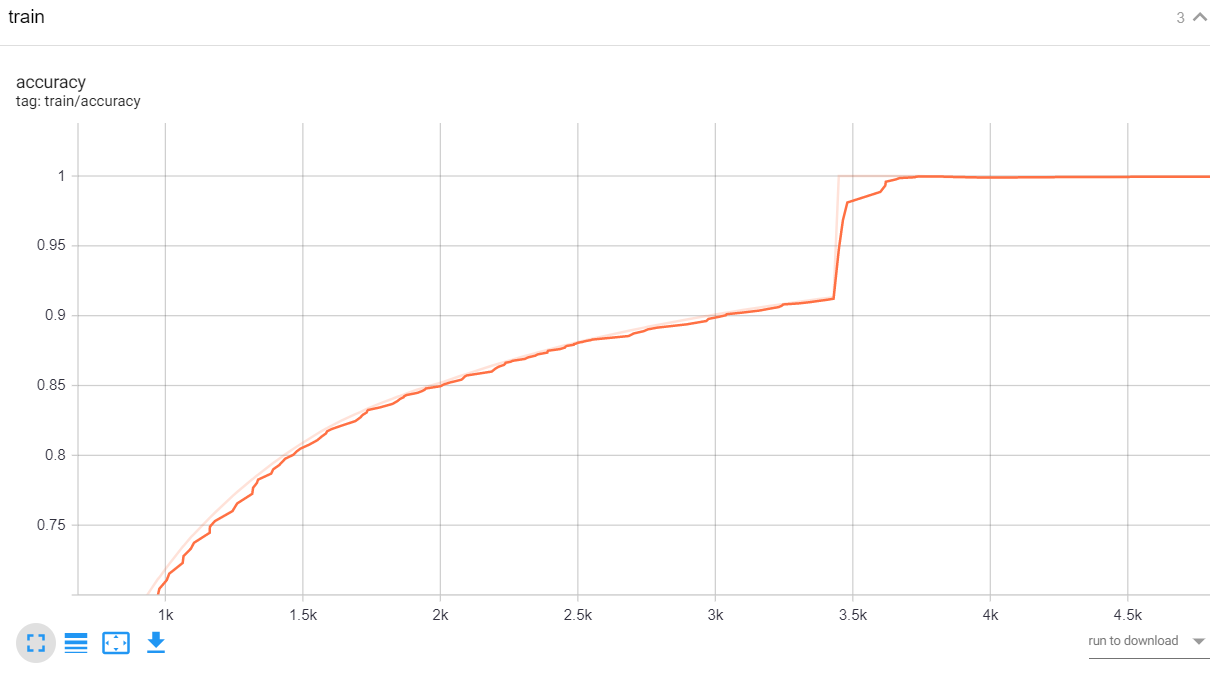
\includegraphics[width=1.1\textwidth]{pic/ResNetmnisttrain.png}
        \end{minipage}
    }
    \subfigure[Res-leap-gray]{
        \begin{minipage}[b]{0.3\textwidth}
            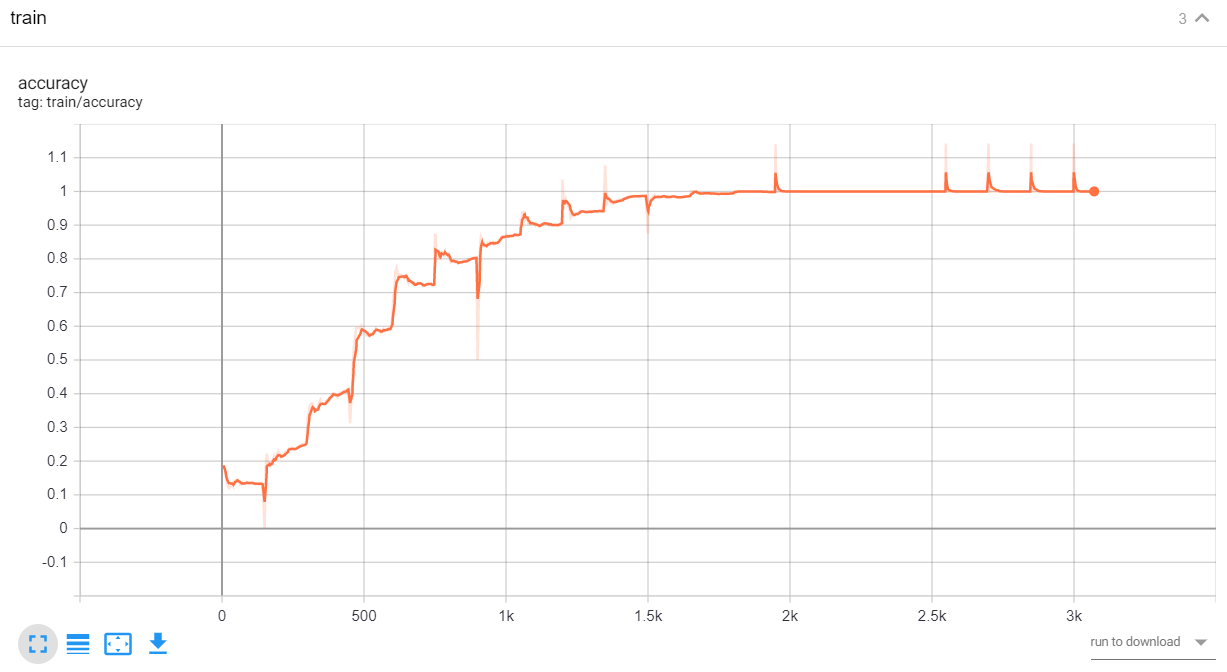
\includegraphics[width=1.1\textwidth]{pic/ResNetleaptrain.png}
        \end{minipage}
    }
    \subfigure[Res-leap-RGB]{
        \begin{minipage}[b]{0.3\textwidth}
            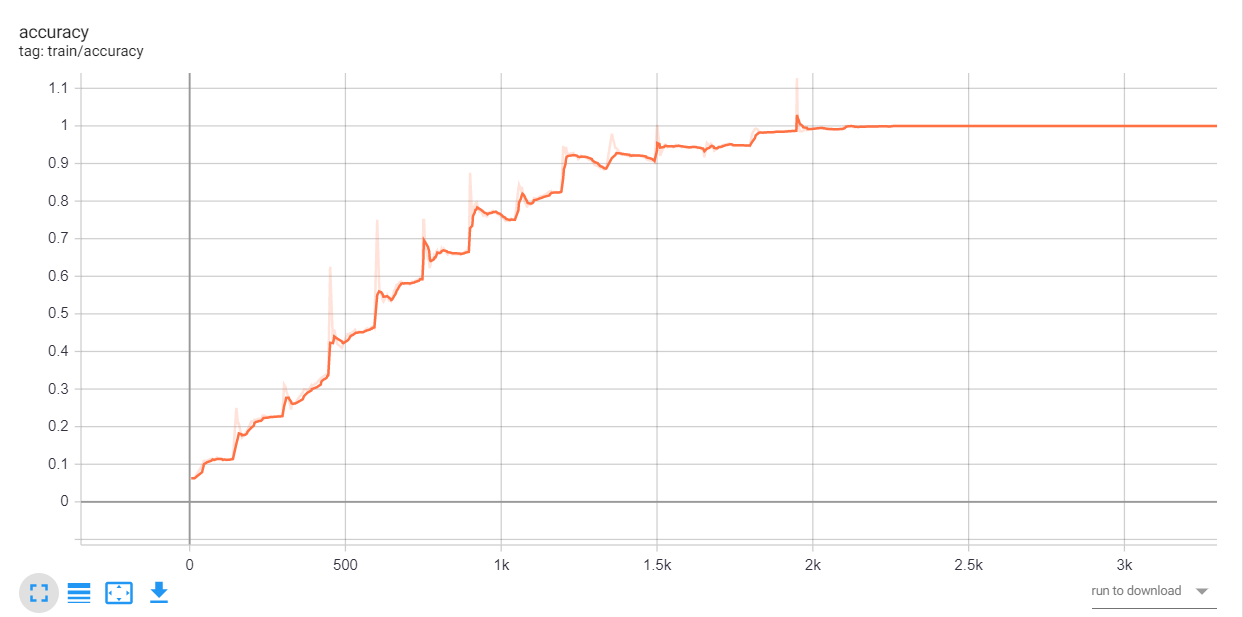
\includegraphics[width=1.1\textwidth]{pic/ResNetleaprgbtrain.png}
        \end{minipage}
    }


    \caption{Variation of the accuracy during the training process.}
\end{figure}

\begin{figure}[H]
    \centering

    \subfigure[Le-MNIST-gray]{
        \begin{minipage}[b]{0.3\textwidth}
            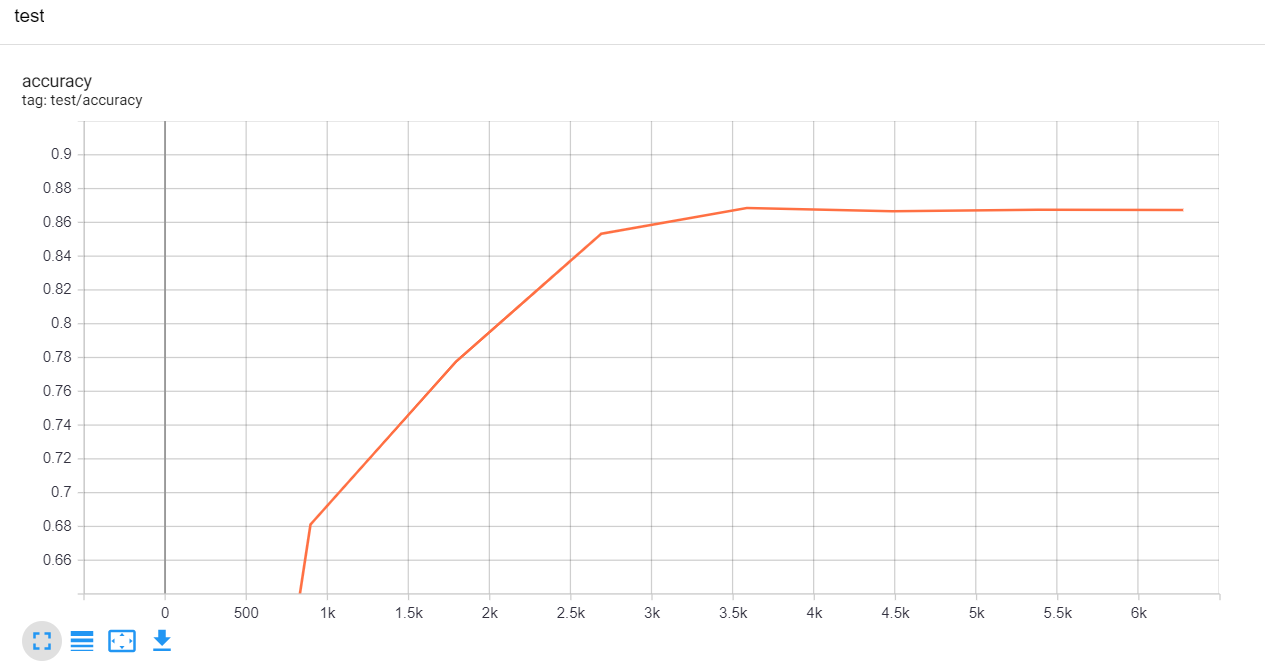
\includegraphics[width=1.1\textwidth]{pic/LeNet5GraymnistTest.png}
        \end{minipage}
    }
    \subfigure[Le-leap-gray]{
        \begin{minipage}[b]{0.3\textwidth}
            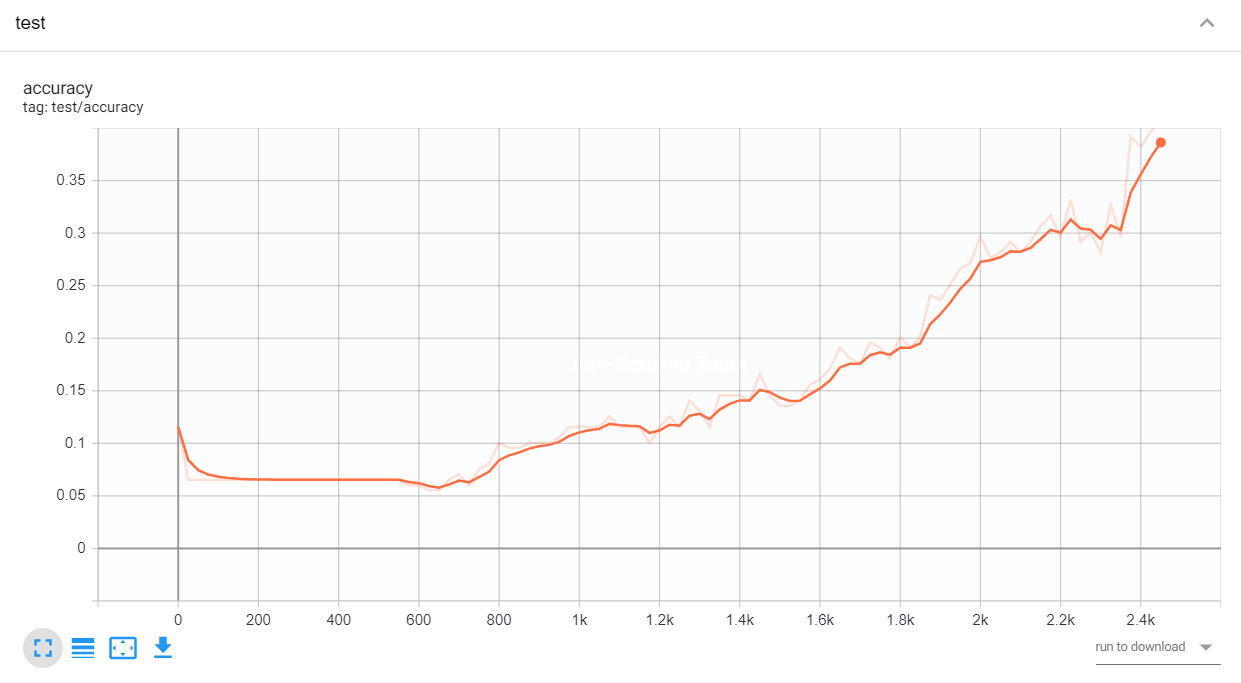
\includegraphics[width=1.1\textwidth]{pic/LeNet5grayleaptest.png}
        \end{minipage}
    }
    \subfigure[Le-leap-RGB]{
        \begin{minipage}[b]{0.3\textwidth}
            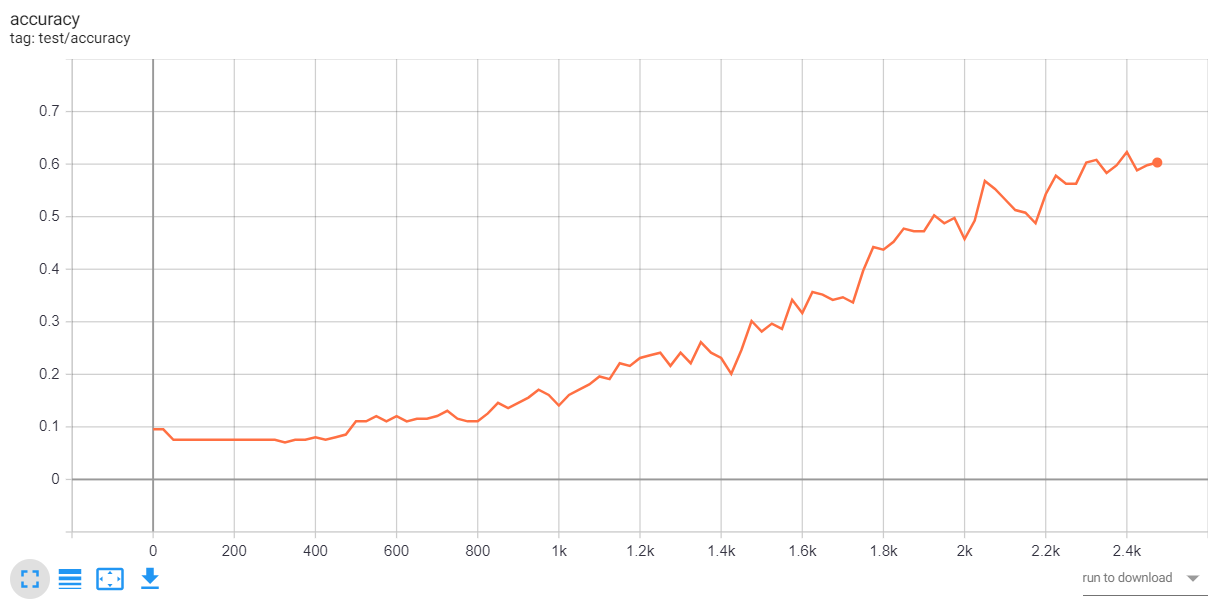
\includegraphics[width=1.\textwidth]{pic/LeNet5leaprgbtest.png}
        \end{minipage}
    }
    \\
    \subfigure[Res-MNIST-gray]{
        \begin{minipage}[b]{0.3\textwidth}
            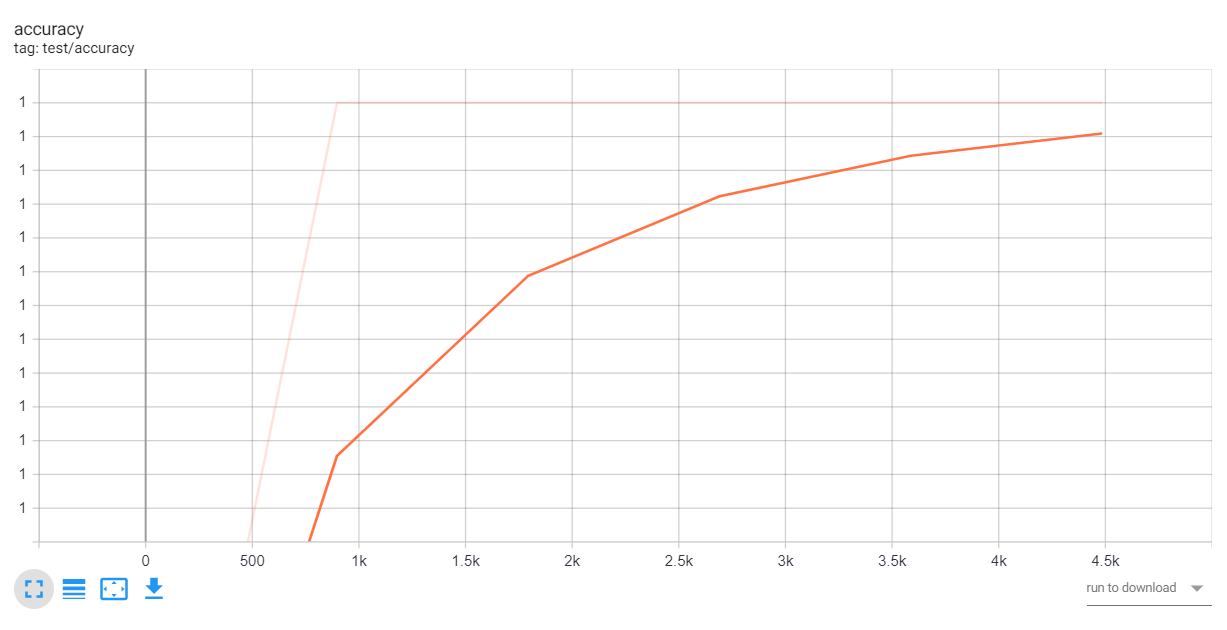
\includegraphics[width=1.1\textwidth]{pic/ResNetmnisttest.png}
        \end{minipage}
    }
    \subfigure[Res-leap-gray]{
        \begin{minipage}[b]{0.3\textwidth}
            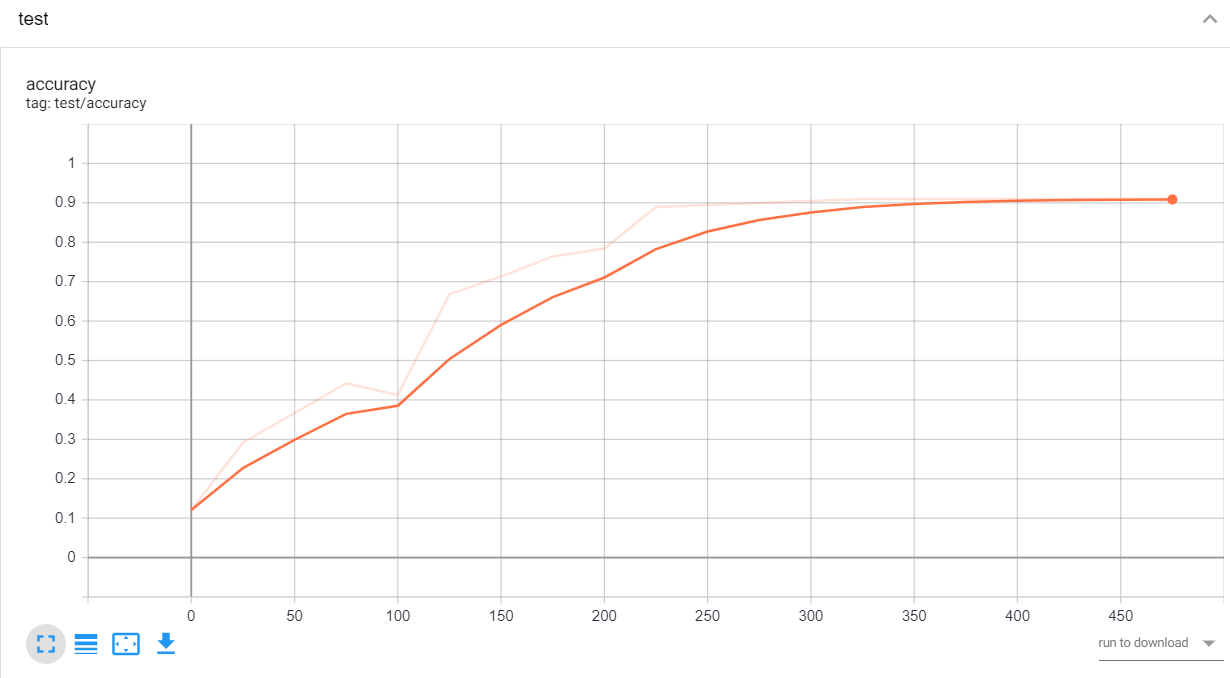
\includegraphics[width=1.1\textwidth]{pic/ResNetleaptest.png}
        \end{minipage}
    }
    \subfigure[Res-leap-RGB]{
        \begin{minipage}[b]{0.3\textwidth}
            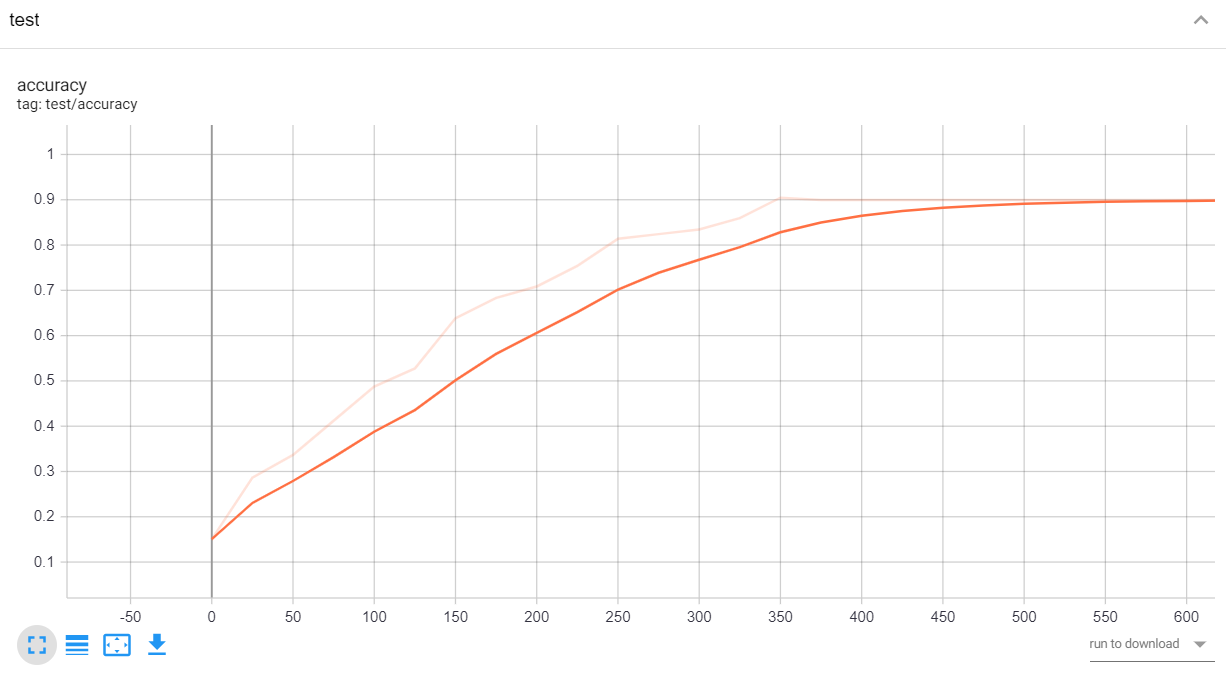
\includegraphics[width=1.1\textwidth]{pic/ResNetleaprgbtest.png}
        \end{minipage}
    }


    \caption{Variation of the accuracy during the testing process.}
\end{figure}

As we can see in the above, the first group of charts shows how the loss variate in the training process with different settings. For LeNet5, there is a clearly slowdown on the speed of the loss reduction. pic(a) shows that when dealing with the MNIST dataset, LeNet5 can reduce the loss to almost zero within 15k images. But for kinect leap dataset with larger scale of images, LeNet5 can not do so well. When the amount of fed images comes to 15k, the loss only reduced to around 1.2, which is actually an unacceptable performance. The result is getting a little better when we change the images into RGB format, loss can fall around 0.5. 

Respectively, the accuracy performances under each settings are highly corresponding to the loss reduction. So, imaginablely, accuracy when LeNet5 dealing with the MNIST dataset is actually pretty well that can reach 100\% in training process and 87\% in testing process. But when it came to kinect leap dataset, the even the training accuracy can only reach 55\% and the testing accuracy is no more than 40\%. The RGB images setting basicly shares the same result. 

The performance of ResNet34 shows much better performance on both datasets. On sign language mnist dataset, loss can be reduced to almost zero around 3.5k. When facing the kinect leap dataset, ResNet34 surprisingly did even better than on MNIST dataset. Loss reaches almost 0 before 2k. For RGB images ResNet34 take 0.5k more images to reach the same level.

The result are also pretty well for accuracy. In the training process, all accuracy can reach 100\%. And for test process ResNet34 can also reach 90\% accuracy which is relatively higher than the performance of LeNet5.

In conclusion, we can say that there is no doubt that ResNet34 shows a better performance. And for gray scale, this attribute has raletively low affect on the final result. Since every gray scale image is actually generate from an RGB image, we can say that each gray scale image mentains enough information from gray sacle images. LeNet5 shows poor performance compared to ResNet34, espacially on the large scale image. But one of its advantages is that the small scale of this network, which leads to a smaller computational resource.

\section{Application}
After training our network, to make the user more convenient to use our network to get the gesture recognition result, we use python to create a product to give the answer.

This product can automatically choose the best model to do the prediction work by analyze the image itself. In the previous part, we find out that different model may have different performance when predict different image. So, after experiment, we set serval thresholds to judge the image and then choose the most suitable model and do prediction. 

After choosing the model, we preprocess the image and then feed it the model to get the prediction result, compare with the ground truth to find out whether the output is correct.

\section{Future Work \& Conclusion}
\subsection{Future Work}
As discussed in the previous section, our project reaches our expecting target basically. However, there are still rooms for improvement. 

As for now, LeNet is more suitable for pictures whose resolution are lower than 28×28 with faster calculation and less occupation in space. ResNet works better on larger images with deeper model and longer training time. In daily applications, however, most cases require to work on larger images. In that case, we need to improve the algorithm to work faster on these images. We are aware that there are various existing methods and techniques to improve ResNet and that is exactly what we need to work on in the future.

Our project can now recognize static images, but in most cases, it is dynamic recognition that truly takes place. For this part, we still need to learn how to draw frame from a video and combine several images together to recognize gestures.

\subsection{Work}
Our project aims at gesture recognition on numerical gestures. We choose Microsoft Kinect and Leap Motion as our training data and apply LeNet and ResNet as our network model. We successfully finish the training and testing of the two chosen networks and compare the performance between the two neural networks. We also implement a final product that can perform as an App to recognize gestures using our algorithm.


\end{document}


